%%%%%%%%%% EJERCICIO 2 %%%%%%%%%%
\newpage
\begin{ejer}
    \textbf{Ejercicio 2. Un ejemplo clásico de red social de tamaño pequeño es el de las familias 
    más influyentes en la política, la economía y la vida social de la Florencia del siglo XV. 
    Los historiadores John Padgett y Christopher Ansell estudiaron esta red social en 1993, 
    basándose en datos tomados de archivos históricos (ver el artículo [2], que se ha adjuntado en 
    Recursos del aula virtual). El grafo que representa dicha red social, que no es dirigido, 
    y se forma dibujando una arista entre dos familias cada vez que un matrimonio las vincula, es el siguiente:}
\end{ejer}
\addcontentsline{toc}{subsection}{Ejercicio 2}
 %%% IMAGEN DE FAMILIAS INFLUYENTES %%%
 \begin{figure}[H]
	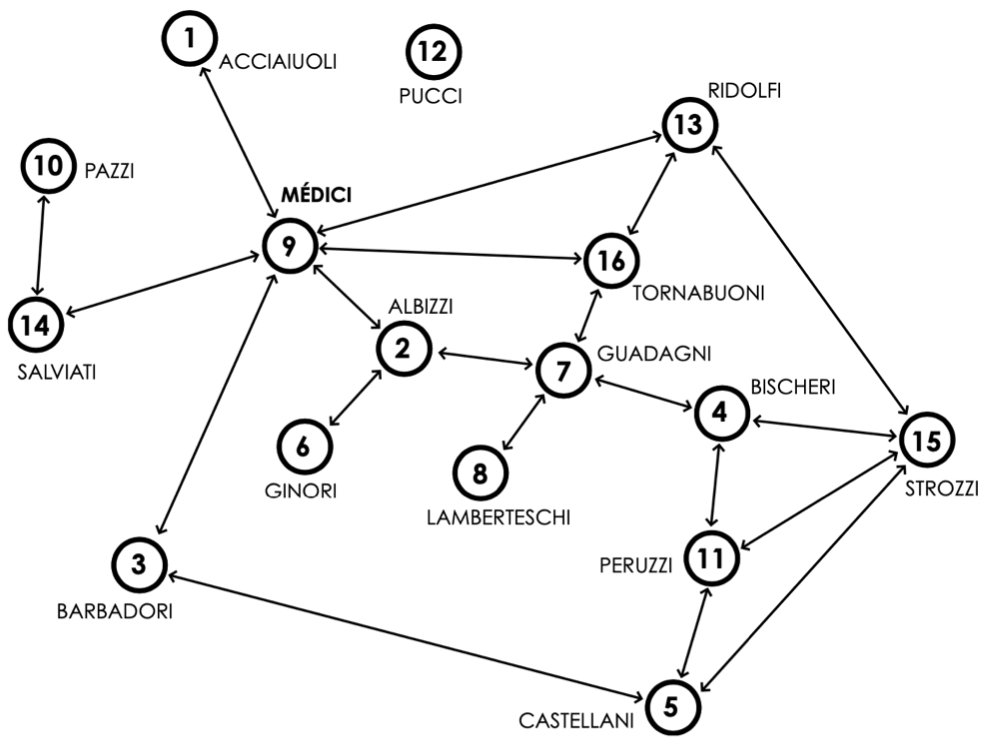
\includegraphics[width=\textwidth/2]{familiasInfluyentes}
	\centering
	\caption{Familias influyentes de Florencia.}
    \label{fig:familiasInfluyentes}
\end{figure}
\begin{ejer}
    \textbf{A simple vista se observa que la familia Médici, con el vértice $9$, ocupa una posición central, pues ostenta el grado máximo. 
    Los autores del estudio conjeturaron que los Médici alcanzaron una posición de dominio en la sociedad florentina precisamente forzando 
    su alianza con el resto de familias a través de múltiples matrimonios.}
\end{ejer}
%%%%%%%%%%%%%%%%%%%%%%%%%%%%%%%%%%%%%%%%%%%%%%%%%%%%%%%    APARTADO_1   %%%%%%%%%%%%%%%%%%%%%%%%%%%%%%%%%%%%%%%%%%%%%%%%%%%%%%%%%%%%%%%
\begin{ejer}
    \begin{itemize}
        \item \textbf{Aplica el algoritmo PageRank a esta red social para confirmar que, en efecto, la familia Médici era la más relevante en esta pequeña red social.}
    \end{itemize}
\end{ejer}
\addcontentsline{toc}{subsubsection}{Apartado 1}
\begin{sagecommandline}
    sage: N = matrix(RDF,[[0, 0, 0, 0, 0, 0, 0, 0, 1, 0, 0, 0, 0, 0, 0, 0],[0, 0, 0, 0, 0, 1/3, 1/3, 0, 1/3, 0, 0, 0, 0, 0, 0, 0],[0, 0, 0, 0, 1/2, 0, 0, 0, 1/2, 0, 0, 0, 0, 0, 0, 0],[0, 0, 0, 0, 0, 0, 1/3, 0, 0, 0, 1/3, 0, 0, 0, 1/3, 0],[0, 0, 1/3, 0, 0, 0, 0, 0, 0, 0, 1/3, 0, 0, 0, 1/3, 0],[0, 1, 0, 0, 0, 0, 0, 0, 0, 0, 0, 0, 0, 0, 0, 0],[0, 1/4, 0, 1/4, 0 , 0, 0, 1/4, 0, 0, 0, 0, 0, 0, 0,1/4],[0, 0, 0, 0, 0, 0, 1, 0, 0, 0, 0, 0, 0, 0, 0, 0],[1/6, 1/6, 1/6, 0, 0 , 0, 0, 0, 0, 1/6, 0, 0, 1/6, 1/6, 0, 0],[0, 0, 0, 0, 0, 0, 0, 0, 0, 0, 0, 0, 0, 1, 0, 0],[0, 0, 0, 1/2, 1/2 , 0, 0, 0, 0, 0, 0, 0, 0, 0, 0, 0],[0, 0, 0, 0, 0, 0, 0, 0, 0, 0, 0, 0, 0, 0, 0, 0],[0, 0, 0, 0, 0, 0, 0, 0, 1/3, 0, 0, 0, 0, 0, 1/3, 1/3],[0, 0, 0, 0, 0, 0, 0, 0, 1/2, 1/2, 0, 0, 0, 0, 0, 0],[0, 0, 0, 1/4, 1/4, 0, 0, 0, 0, 0, 1/4, 0, 1/4, 0, 0, 0],[0, 0, 0, 0, 0, 0, 1/3, 0, 1/3, 0, 0, 0, 1/3, 0, 0, 0]])
\end{sagecommandline}
\resizebox{\textwidth}{!}{$
    N(x)= \sage{N}
$}
\par $N(x)$ representa la matriz de transición de la red descrita anteriormente.

\par \textbf{El primer paso} es crear una matriz estocástica $Q(x)$, que sirve para asegurarnos de que el camino
aleatorio llega a todas las familias de la red social. Para ello, observo la matriz inicial y añado en la fila
que no tiene ningún enlace de salida (por tanto un nodo colgante) el valor $1/n^o nodos$ a todas sus columnas para indicar que 
a todos los nodos, incluido el mismo, se puede llegar con la misma aleatoridad y de manera uniforme. 

\begin{sagecommandline}
    sage: Q = matrix(RDF,[[0, 0, 0, 0, 0, 0, 0, 0, 1, 0, 0, 0, 0, 0, 0, 0],[0, 0, 0, 0, 0, 1/3, 1/3, 0, 1/3, 0, 0, 0, 0, 0, 0, 0],[0, 0, 0, 0, 1/2, 0, 0, 0, 1/2, 0, 0, 0, 0, 0, 0, 0],[0, 0, 0, 0, 0, 0, 1/3, 0, 0, 0, 1/3, 0, 0, 0, 1/3, 0],[0, 0, 1/3, 0, 0, 0, 0, 0, 0, 0, 1/3, 0, 0, 0, 1/3, 0],[0, 1, 0, 0, 0, 0, 0, 0, 0, 0, 0, 0, 0, 0, 0, 0],[0, 1/4, 0, 1/4, 0 , 0, 0, 1/4, 0, 0, 0, 0, 0, 0, 0,1/4],[0, 0, 0, 0, 0, 0, 1, 0, 0, 0, 0, 0, 0, 0, 0, 0],[1/6, 1/6, 1/6, 0, 0 , 0, 0, 0, 0, 1/6, 0, 0, 1/6, 1/6, 0, 0],[0, 0, 0, 0, 0, 0, 0, 0, 0, 0, 0, 0, 0, 1, 0, 0],[0, 0, 0, 1/2, 1/2 , 0, 0, 0, 0, 0, 0, 0, 0, 0, 0, 0],[1/16, 1/16, 1/16, 1/16, 1/16, 1/16, 1/16, 1/16, 1/16, 1/16, 1/16, 1/16, 1/16, 1/16, 1/16, 1/16],[0, 0, 0, 0, 0, 0, 0, 0, 1/3, 0, 0, 0, 0, 0, 1/3, 1/3],[0, 0, 0, 0, 0, 0, 0, 0, 1/2, 1/2, 0, 0, 0, 0, 0, 0],[0, 0, 0, 1/4, 1/4, 0, 0, 0, 0, 0, 1/4, 0, 1/4, 0, 0, 0],[0, 0, 0, 0, 0, 0, 1/3, 0, 1/3, 0, 0, 0, 1/3, 0, 0, 0]])
\end{sagecommandline}
\resizebox{\textwidth}{!}{$
    Q(x)= \sage{Q}
$}

\par \textbf{El segundo paso}, es obtener la matriz de transición de PageRank $P=pQ + (1-p)A$ para resolver el 
problema de que se atasque en pequeños subgrafos de la red.
\par Donde:
\begin{itemize}
    \item $Q$ es la matriz obtenida en el paso anterior.
    \item $A$ es la matriz ($n^onodos \times n^onodos$), donde todos los nodos están conectados entre sí y cuyas 
    entradas son $1/n^o nodos$.
    \begin{sagecommandline}
        sage: A = matrix(RDF,[[1/16, 1/16, 1/16, 1/16, 1/16, 1/16, 1/16, 1/16, 1/16, 1/16, 1/16, 1/16, 1/16, 1/16, 1/16, 1/16],[1/16, 1/16, 1/16, 1/16, 1/16, 1/16, 1/16, 1/16, 1/16, 1/16, 1/16, 1/16, 1/16, 1/16, 1/16, 1/16],[1/16, 1/16, 1/16, 1/16, 1/16, 1/16, 1/16, 1/16, 1/16, 1/16, 1/16, 1/16, 1/16, 1/16, 1/16, 1/16],[1/16, 1/16, 1/16, 1/16, 1/16, 1/16, 1/16, 1/16, 1/16, 1/16, 1/16, 1/16, 1/16, 1/16, 1/16, 1/16],[1/16, 1/16, 1/16, 1/16, 1/16, 1/16, 1/16, 1/16, 1/16, 1/16, 1/16, 1/16, 1/16, 1/16, 1/16, 1/16],[1/16, 1/16, 1/16, 1/16, 1/16, 1/16, 1/16, 1/16, 1/16, 1/16, 1/16, 1/16, 1/16, 1/16, 1/16, 1/16],[1/16, 1/16, 1/16, 1/16, 1/16, 1/16, 1/16, 1/16, 1/16, 1/16, 1/16, 1/16, 1/16, 1/16, 1/16, 1/16],[1/16, 1/16, 1/16, 1/16, 1/16, 1/16, 1/16, 1/16, 1/16, 1/16, 1/16, 1/16, 1/16, 1/16, 1/16, 1/16],[1/16, 1/16, 1/16, 1/16, 1/16, 1/16, 1/16, 1/16, 1/16, 1/16, 1/16, 1/16, 1/16, 1/16, 1/16, 1/16],[1/16, 1/16, 1/16, 1/16, 1/16, 1/16, 1/16, 1/16, 1/16, 1/16, 1/16, 1/16, 1/16, 1/16, 1/16, 1/16],[1/16, 1/16, 1/16, 1/16, 1/16, 1/16, 1/16, 1/16, 1/16, 1/16, 1/16, 1/16, 1/16, 1/16, 1/16, 1/16],[1/16, 1/16, 1/16, 1/16, 1/16, 1/16, 1/16, 1/16, 1/16, 1/16, 1/16, 1/16, 1/16, 1/16, 1/16, 1/16],[1/16, 1/16, 1/16, 1/16, 1/16, 1/16, 1/16, 1/16, 1/16, 1/16, 1/16, 1/16, 1/16, 1/16, 1/16, 1/16],[1/16, 1/16, 1/16, 1/16, 1/16, 1/16, 1/16, 1/16, 1/16, 1/16, 1/16, 1/16, 1/16, 1/16, 1/16, 1/16],[1/16, 1/16, 1/16, 1/16, 1/16, 1/16, 1/16, 1/16, 1/16, 1/16, 1/16, 1/16, 1/16, 1/16, 1/16, 1/16],[1/16, 1/16, 1/16, 1/16, 1/16, 1/16, 1/16, 1/16, 1/16, 1/16, 1/16, 1/16, 1/16, 1/16, 1/16, 1/16]])
    \end{sagecommandline} 
    \resizebox{\textwidth}{!}{$
        A(x)= \sage{A}
    $}
    \begin{sagecommandline}
        sage: GA = Graph(A, multiedges=True)
        sage: Aplot = GA.plot()
    \end{sagecommandline}
    
    %%% GRAFO DE RED SIMPLIFICADA %%%
    \begin{figure}[H]
        \sageplot[scale=.6]{Aplot, axes=False}
        \centering
        \label{redA_2}
        \caption{Red A donde todos los nodos están conectados entre sí.}
    \end{figure}
    \item $p$ es el factor de amortiguamiento propuesto por Brin y Page (1998) que tiene que ser un valor 
    comprendido entre [0..1], en este caso particular establezco $p=0.85$.
    \begin{sagecommandline}
        sage: factor=0.85
    \end{sagecommandline}
    \item  $(1-p)$ es la probabilidad de que una persona decida no ser influenciada por ninguna familia enlazada por la familia donde se encuentra y 
    decida navegar a una nueva y aleatoria dentro de la red. Por otro lado, con probabilidad $p$, sigue a las familias enlazadas 
    como de costumbre.
    \begin{sagecommandline}
        sage: prob_nueva_pagina=1-factor
        sage: prob_enlace=factor
    \end{sagecommandline}
\end{itemize}

\par Con estos parámetros se obtiene la matriz $P$ estocástica.
\begin{sagecommandline}
    sage: P=prob_enlace*Q+prob_nueva_pagina*A
\end{sagecommandline}
\resizebox{\textwidth}{!}{$
    P(x)= \sage{P}
$}

\par \textbf{El tercer paso} es obtener el camino aleatorio que es la matriz por columnas de los autovectores de $P$.
Para ello, muestro los vectores propios de la matriz $P$ y asigno cada autovector.
\begin{sagecommandline}[\textwidth]
    sage: P.eigenvectors_right()
\end{sagecommandline}
    
\begin{sagecommandline}
    sage: q1=(P.eigenvectors_right()[0])[1][0];
\end{sagecommandline}
\resizebox{\textwidth}{!}{$
    q1= \sage{q1}
$}

\begin{sagecommandline}
    sage: q2=(P.eigenvectors_right()[1])[1][0];
\end{sagecommandline}
\resizebox{\textwidth}{!}{$
    q2= \sage{q2}
$}

\begin{sagecommandline}
    sage: q3=(P.eigenvectors_right()[2])[1][0];
\end{sagecommandline}
\resizebox{\textwidth}{!}{$
    q3= \sage{q3}
$}

\begin{sagecommandline}
    sage: q4=(P.eigenvectors_right()[3])[1][0];
\end{sagecommandline}
\resizebox{\textwidth}{!}{$
    q4= \sage{q4}
$}

\begin{sagecommandline}
    sage: q5=(P.eigenvectors_right()[4])[1][0];
\end{sagecommandline}
\resizebox{\textwidth}{!}{$
    q5= \sage{q5}
$}

\begin{sagecommandline}
    sage: q6=(P.eigenvectors_right()[5])[1][0];
\end{sagecommandline}
\resizebox{\textwidth}{!}{$
    q6= \sage{q6}
$}

\begin{sagecommandline}
    sage: q7=(P.eigenvectors_right()[6])[1][0];
\end{sagecommandline}
\resizebox{\textwidth}{!}{$
    q7= \sage{q7}
$}

\begin{sagecommandline}
    sage: q8=(P.eigenvectors_right()[7])[1][0];
\end{sagecommandline}
\resizebox{\textwidth}{!}{$
    q8= \sage{q8}
$}

\begin{sagecommandline}
    sage: q9=(P.eigenvectors_right()[8])[1][0];
\end{sagecommandline}
\resizebox{\textwidth}{!}{$
    q9= \sage{q9}
$}

\begin{sagecommandline}
    sage: q10=(P.eigenvectors_right()[9])[1][0];
\end{sagecommandline}
\resizebox{\textwidth}{!}{$
    q10= \sage{q10}
$}

\begin{sagecommandline}
    sage: q11=(P.eigenvectors_right()[10])[1][0];
\end{sagecommandline}
\resizebox{\textwidth}{!}{$
    q11= \sage{q11}
$}

\begin{sagecommandline}
    sage: q12=(P.eigenvectors_right()[11])[1][0];
\end{sagecommandline}
\resizebox{\textwidth}{!}{$
    q12= \sage{q12}
$}

\begin{sagecommandline}
    sage: q13=(P.eigenvectors_right()[12])[1][0];
\end{sagecommandline}
\resizebox{\textwidth}{!}{$
    q13= \sage{q13}
$}

\begin{sagecommandline}
    sage: q14=(P.eigenvectors_right()[13])[1][0];
\end{sagecommandline}
\resizebox{\textwidth}{!}{$
    q14= \sage{q14}
$}

\begin{sagecommandline}
    sage: q15=(P.eigenvectors_right()[14])[1][0];
\end{sagecommandline}
\resizebox{\textwidth}{!}{$
    q15= \sage{q15}
$}

\begin{sagecommandline}
    sage: q16=(P.eigenvectors_right()[15])[1][0];
\end{sagecommandline}
\resizebox{\textwidth}{!}{$
    q16= \sage{q16}
$}

\par El camino aleatorio resultante $Q_C$ es asociable, aperiódico e irreducible.

\begin{sagecommandline}
    sage: Q_C=column_matrix([q1,q2,q3,q4,q5,q6,q7,q8,q9,q10,q11,q12,q13,q14,q15,q16]);
\end{sagecommandline}
\resizebox{\textwidth}{!}{$
    Q_C= \sage{Q_C}
$}

\begin{sagecommandline}
    sage: GQ = DiGraph(Q_C, multiedges=True)
    sage: Qplot = GQ.plot()
\end{sagecommandline}
%%% GRAFO DE RED SIMPLIFICADA %%%
\begin{figure}[H]
    \sageplot[scale=.5]{Qplot, axes=False}
    \centering
    \label{caminoZ_2}
    \caption{Camino aleatorio resultante es asociable, aperiódico e irreducible.}
\end{figure}

\par \textbf{El cuarto paso} es obtener la matriz donde la diagonal tiene los valores propios de $P$.
\par Obtengo los valores propios de la matriz $P$.
\begin{sagecommandline}
    sage: P_valores_propios = P.eigenvalues()
\end{sagecommandline}
\resizebox{\textwidth}{!}{$
    Valores propios: \sage{P_valores_propios}
$}

\par $D$ es la matriz donde la diagonal tiene los valores propios de $P$.
\begin{sagecommandline}
    sage: D = diagonal_matrix([P.eigenvalues()[0],P.eigenvalues()[1],P.eigenvalues()[2],P.eigenvalues()[3],P.eigenvalues()[4],P.eigenvalues()[5],P.eigenvalues()[6],P.eigenvalues()[7],P.eigenvalues()[8],P.eigenvalues()[9],P.eigenvalues()[10],P.eigenvalues()[11],P.eigenvalues()[12],P.eigenvalues()[13],P.eigenvalues()[14],P.eigenvalues()[15]])
\end{sagecommandline}
\resizebox{\textwidth}{!}{$
    D= \sage{D}
$}

\par \textbf{Por último}, calculo el \texttt{PageRank} de una familia en la red que es la probabilidad estacionaria de esa familia.
\par Calculo primero la matriz estacionaria, sin importar por que nodo empiece.
\begin{sagecommandline}
    sage: mo=matrix(RDF,[1, 0, 0, 0, 0, 0, 0, 0, 0, 0, 0, 0, 0, 0, 0, 0])
\end{sagecommandline}
\par $\mu^{(100)} = \mu^{(0)} \cdot P^{(100)} = \mu^{(0)} \cdot Q_C \cdot D^{(100)} \cdot Q_C^{(-1)}$
\begin{sagecommandline}
    sage: mo*Q_C*D^100*Q_C.inverse()
\end{sagecommandline}
\begin{sagecommandline}
    sage: z=(0.030616772148504806,0.07626307878565806, 0.05150657580871245, 0.07070219766081234, 0.0737287188007328, 0.031508862421612535, 0.08877069919427012, 0.02876476367779198, 0.14622904976114215, 0.06830356213169397, 0.06509509970488973, 0.00990099009900966, 0.05766828706625104, 0.08867479996044474, 0.06716243109855179, 0.04510411167989654)
\end{sagecommandline}

\par Compruebo que la suma de todas las probabilidades estacionarias de las páginas da aproximadamente 1.
\begin{sagecommandline}
    sage: sum(z)
\end{sagecommandline}

\par A partir de los datos obtenidos, he creado esta tabla \ref{fig:pageRankFamilias-1} donde se puede ver claramente que 
la familia más influente es \texttt{Médici} porque su \texttt{PageRank} es 0.14622904976114215 y la que menos es 
\texttt{Pucci} porque su \texttt{PageRank} es 0.00990099009900966.
\par El orden de relevancia es el siguiente : Médici, Guadagni, Salviati, Albizzi, Castellani, Bischeri, Pazzi, Strozzi, Peruzzi,
Ridolfi, Barbadori, Tornabuoni, Ginori, Acciaiuoli, Lamberteschi y Pucci.

\begin{figure}[H]
    \centering
    \begin{tabular}{|c|c|c|}
        \hline
        \rowcolor{azul} \multicolumn{2}{|c|}{\textbf{Familia}}& \\ \hline
        \rowcolor{azul} \textbf{Número} & \textbf{Nombre} & \textbf{PageRank} \\ \hline
        1 & Acciaiuoli & \cellcolor{orange!25}{0.030616772148504806} \\ \hline
        2 & Albizzi & \cellcolor{blue!25}{0.07626307878565806} \\ \hline
        3 & Barbadori & \cellcolor{yellow!25}{0.05150657580871245} \\ \hline
        4 & Bischeri & \cellcolor{violet!25}{0.07070219766081234} \\ \hline
        5 & Castellani & \cellcolor{blue!25}{0.0737287188007328} \\ \hline
        6 & Ginori & \cellcolor{orange!25}{0.031508862421612535} \\ \hline
        7 & Guadagni & \cellcolor{blue!25}{0.08877069919427012} \\ \hline
        8 & Lamberteschi & \cellcolor{orange!25}{0.02876476367779198} \\ \hline
        9 & Médici & \cellcolor{green!25}{0.14622904976114215} \\ \hline
        10 & Pazzi & \cellcolor{violet!25}{0.06830356213169397} \\ \hline
        11 & Peruzzi & \cellcolor{violet!25}{0.06509509970488973} \\ \hline
        12 & Pucci & \cellcolor{red!25}{0.00990099009900966} \\ \hline
        13 & Ridolfi & \cellcolor{yellow!25}{0.05766828706625104} \\ \hline
        14 & Salviati & \cellcolor{blue!25}{0.08867479996044474} \\ \hline
        15 & Strozzi & \cellcolor{violet!25}{0.06716243109855179} \\ \hline
        16 & Tornabuoni & \cellcolor{yellow!25}{0.04510411167989654} \\ \hline
    \end{tabular}
    \caption{PageRank de las familias de la red.}
    \label{fig:pageRankFamilias-1}
\end{figure}
%%%%%%%%%%%%%%%%%%%%%%%%%%%%%%%%%%%%%%%%%%%%%%%%%%%%%%%%%%%%%%%%%%%%%%%%%%%%%%%%%%%%%%%%%%%%%%%%%%%%%%%%%%%%%%%%%%%%%%%%%%%%%%%%%%%%%%%
%%%%%%%%%%%%%%%%%%%%%%%%%%%%%%%%%%%%%%%%%%%%%%%%%%%%%%%    APARTADO_2   %%%%%%%%%%%%%%%%%%%%%%%%%%%%%%%%%%%%%%%%%%%%%%%%%%%%%%%%%%%%%%%
\begin{ejer}
    \begin{itemize}
        \item \textbf{Repite el apartado anterior, tomando ahora $p = 0.8ab$ y $p = 0.6ab$, donde $ab$ son las dos últimas cifras de tu DNI. ¿Varía mucho el resultado? ¿Por qué?}
    \end{itemize}
\end{ejer}
\addcontentsline{toc}{subsubsection}{Apartado 2}
\par\textbf{Caso 1: $p = 0.889$}
\par Obtengo otra vez la matriz de transición de PageRank $P=pQ + (1-p)A$ para resolver el 
problema de que se atasque en pequeños subgrafos de la red.
\par Donde:
\begin{itemize}
    \item $p$ es el factor de amortiguamiento propuesto por Brin y Page (1998) que tiene que ser un valor 
    comprendido entre [0..1], tomando ahora $p = 0.889$, puesto que mi DNI acaba en 89.
    \begin{sagecommandline}
        sage: factor=0.889
        sage: prob_nueva_pagina=1-factor
        sage: prob_enlace=factor
    \end{sagecommandline}
\end{itemize}

\par Con estos parámetros se obtiene la matriz $P$ estocástica.
\begin{sagecommandline}
    sage: P=prob_enlace*Q+prob_nueva_pagina*A
\end{sagecommandline}
\resizebox{\textwidth}{!}{$
    P(x)= \sage{P}
$}

\par \textbf{El tercer paso} es obtener el camino aleatorio que es la matriz por columnas de los autovectores de $P$.
Para ello, muestro los vectores propios de la matriz $P$ y asigno cada autovector.
\begin{sagecommandline}[\textwidth]
    sage: P.eigenvectors_right()
\end{sagecommandline}

  
\begin{sagecommandline}
    sage: q1=(P.eigenvectors_right()[0])[1][0];
\end{sagecommandline}
\resizebox{\textwidth}{!}{$
    q1= \sage{q1}
$}

\begin{sagecommandline}
    sage: q2=(P.eigenvectors_right()[1])[1][0];
\end{sagecommandline}
\resizebox{\textwidth}{!}{$
    q2= \sage{q2}
$}

\begin{sagecommandline}
    sage: q3=(P.eigenvectors_right()[2])[1][0];
\end{sagecommandline}
\resizebox{\textwidth}{!}{$
    q3= \sage{q3}
$}

\begin{sagecommandline}
    sage: q4=(P.eigenvectors_right()[3])[1][0];
\end{sagecommandline}
\resizebox{\textwidth}{!}{$
    q4= \sage{q4}
$}

\begin{sagecommandline}
    sage: q5=(P.eigenvectors_right()[4])[1][0];
\end{sagecommandline}
\resizebox{\textwidth}{!}{$
    q5= \sage{q5}
$}

\begin{sagecommandline}
    sage: q6=(P.eigenvectors_right()[5])[1][0];
\end{sagecommandline}
\resizebox{\textwidth}{!}{$
    q6= \sage{q6}
$}

\begin{sagecommandline}
    sage: q7=(P.eigenvectors_right()[6])[1][0];
\end{sagecommandline}
\resizebox{\textwidth}{!}{$
    q7= \sage{q7}
$}

\begin{sagecommandline}
    sage: q8=(P.eigenvectors_right()[7])[1][0];
\end{sagecommandline}
\resizebox{\textwidth}{!}{$
    q8= \sage{q8}
$}

\begin{sagecommandline}
    sage: q9=(P.eigenvectors_right()[8])[1][0];
\end{sagecommandline}
\resizebox{\textwidth}{!}{$
    q9= \sage{q9}
$}

\begin{sagecommandline}
    sage: q10=(P.eigenvectors_right()[9])[1][0];
\end{sagecommandline}
\resizebox{\textwidth}{!}{$
    q10= \sage{q10}
$}

\begin{sagecommandline}
    sage: q11=(P.eigenvectors_right()[10])[1][0];
\end{sagecommandline}
\resizebox{\textwidth}{!}{$
    q11= \sage{q11}
$}

\begin{sagecommandline}
    sage: q12=(P.eigenvectors_right()[11])[1][0];
\end{sagecommandline}
\resizebox{\textwidth}{!}{$
    q12= \sage{q12}
$}

\begin{sagecommandline}
    sage: q13=(P.eigenvectors_right()[12])[1][0];
\end{sagecommandline}
\resizebox{\textwidth}{!}{$
    q13= \sage{q13}
$}

\begin{sagecommandline}
    sage: q14=(P.eigenvectors_right()[13])[1][0];
\end{sagecommandline}
\resizebox{\textwidth}{!}{$
    q14= \sage{q14}
$}

\begin{sagecommandline}
    sage: q15=(P.eigenvectors_right()[14])[1][0];
\end{sagecommandline}
\resizebox{\textwidth}{!}{$
    q15= \sage{q15}
$}

\begin{sagecommandline}
    sage: q16=(P.eigenvectors_right()[15])[1][0];
\end{sagecommandline}
\resizebox{\textwidth}{!}{$
    q16= \sage{q16}
$}

\par El camino aleatorio resultante $Q_C$ es asociable, aperiódico e irreducible.

\begin{sagecommandline}
    sage: Q_C=column_matrix([q1,q2,q3,q4,q5,q6,q7,q8,q9,q10,q11,q12,q13,q14,q15,q16]);
\end{sagecommandline}
\resizebox{\textwidth}{!}{$
    Q_C= \sage{Q_C}
$}

\begin{sagecommandline}
    sage: GQ = DiGraph(Q_C, multiedges=True)
    sage: Qplot = GQ.plot()
\end{sagecommandline}
%%% GRAFO DE RED SIMPLIFICADA %%%
\begin{figure}[H]
    \sageplot[scale=.5]{Qplot, axes=False}
    \centering
    \label{caminoZ_2}
    \caption{Camino aleatorio resultante es asociable, aperiódico e irreducible.}
\end{figure}

\par \textbf{El cuarto paso} es obtener la matriz donde la diagonal tiene los valores propios de $P$.
\par Obtengo los valores propios de la matriz $P$.
\begin{sagecommandline}
    sage: P_valores_propios = P.eigenvalues()
\end{sagecommandline}
\resizebox{\textwidth}{!}{$
    Valores propios: \sage{P_valores_propios}
$}

\par $D$ es la matriz donde la diagonal tiene los valores propios de $P$.
\begin{sagecommandline}
    sage: D = diagonal_matrix([P.eigenvalues()[0],P.eigenvalues()[1],P.eigenvalues()[2],P.eigenvalues()[3],P.eigenvalues()[4],P.eigenvalues()[5],P.eigenvalues()[6],P.eigenvalues()[7],P.eigenvalues()[8],P.eigenvalues()[9],P.eigenvalues()[10],P.eigenvalues()[11],P.eigenvalues()[12],P.eigenvalues()[13],P.eigenvalues()[14],P.eigenvalues()[15]])
\end{sagecommandline}
\resizebox{\textwidth}{!}{$
    D= \sage{D}
$}

\par \textbf{Por último}, calculo el \texttt{PageRank} de una familia en la red que es la probabilidad estacionaria de esa familia.
\par Calculo primero la matriz estacionaria, sin importar por que nodo empiece.
\begin{sagecommandline}
    sage: mo=matrix(RDF,[1, 0, 0, 0, 0, 0, 0, 0, 0, 0, 0, 0, 0, 0, 0, 0])
\end{sagecommandline}
\par $\mu^{(100)} = \mu^{(0)} \cdot P^{(100)} = \mu^{(0)} \cdot Q_C \cdot D^{(100)} \cdot Q_C^{(-1)}$
\begin{sagecommandline}
    sage: mo*Q_C*D^100*Q_C.inverse()
\end{sagecommandline}

\begin{sagecommandline}
    sage: z1=(0.029570860773009678, 0.0754079780067131, 0.05158376088937878, 0.07079660905958886, 0.07428425236120793, 0.029691539730023933, 0.08747508847562997, 0.026786980661079315, 0.15000147486369722, 0.07062222025284678, 0.06531503351579934, 0.007345642247369766, 0.05753848456033725, 0.09235401457779774, 0.0673885084397732, 0.04383755158579216)
\end{sagecommandline}

\par Compruebo que la suma de todas las probabilidades estacionarias de las páginas da aproximadamente 1.
\begin{sagecommandline}
    sage: sum(z1)
\end{sagecommandline}

\par A partir de los datos obtenidos, he creado esta tabla \ref{fig:pageRankFamilias-2} donde se puede ver claramente que 
la familia más influente es \texttt{Médici} porque su \texttt{PageRank} es 0.15000147486369722 y la que menos es 
\texttt{Pucci} porque su \texttt{PageRank} es 0.007345642247369766.
\par El orden de relevancia es el siguiente : Médici, Salviati, Guadagni, Albizzi, Castellani, Bischeri, Pazzi, Strozzi, Peruzzi,
Ridolfi, Barbadori, Tornabuoni, Ginori, Acciaiuoli, Lamberteschi y Pucci.

\begin{figure}[H]
    \centering
    \begin{tabular}{|c|c|c|}
        \hline
        \rowcolor{azul} \multicolumn{2}{|c|}{\textbf{Familia}}& \\ \hline
        \rowcolor{azul} \textbf{Número} & \textbf{Nombre} & \textbf{PageRank} \\ \hline
        1 & Acciaiuoli & \cellcolor{orange!25}{0.029570860773009678} \\ \hline
        2 & Albizzi & \cellcolor{blue!25}{0.0754079780067131} \\ \hline
        3 & Barbadori & \cellcolor{yellow!25}{0.05158376088937878} \\ \hline
        4 & Bischeri & \cellcolor{violet!25}{0.07079660905958886} \\ \hline
        5 & Castellani & \cellcolor{blue!25}{0.07428425236120793} \\ \hline
        6 & Ginori & \cellcolor{orange!25}{0.029691539730023933} \\ \hline
        7 & Guadagni & \cellcolor{blue!25}{0.08747508847562997} \\ \hline
        8 & Lamberteschi & \cellcolor{orange!25}{0.026786980661079315} \\ \hline
        9 & Médici & \cellcolor{green!25}{0.15000147486369722} \\ \hline
        10 & Pazzi & \cellcolor{violet!25}{0.07062222025284678} \\ \hline
        11 & Peruzzi & \cellcolor{violet!25}{0.06531503351579934} \\ \hline
        12 & Pucci & \cellcolor{red!25}{0.007345642247369766} \\ \hline
        13 & Ridolfi & \cellcolor{yellow!25}{0.05753848456033725} \\ \hline
        14 & Salviati & \cellcolor{blue!25}{0.09235401457779774} \\ \hline
        15 & Strozzi & \cellcolor{violet!25}{0.0673885084397732} \\ \hline
        16 & Tornabuoni & \cellcolor{yellow!25}{0.04383755158579216} \\ \hline
    \end{tabular}
    \caption{PageRank de las familias de la red.}
    \label{fig:pageRankFamilias-2}
\end{figure}

%%%%%%%%%%%%%%%%%%%%%%%%%%%%%%%%%%%%%%%%%%%%%%%%%%%%%%%%%%%%%%%%%%%%%%%%%%%%%%%%%%%%%%%%%%%%%%%%%%%%%%%%%%%%%%%%%%%%%%%%%%%%%%%%%%%%%%%

\par\textbf{Caso 2: $p = 0.689$}
\par Obtengo otra vez la matriz de transición de PageRank $P=pQ + (1-p)A$ para resolver el 
problema de que se atasque en pequeños subgrafos de la red.
\par Donde:
\begin{itemize}
    \item $p$ es el factor de amortiguamiento propuesto por Brin y Page (1998) que tiene que ser un valor 
    comprendido entre [0..1], tomando ahora $p = 0.689$, puesto que mi DNI acaba en 89.
    \begin{sagecommandline}
        sage: factor=0.689
        sage: prob_nueva_pagina=1-factor
        sage: prob_enlace=factor
    \end{sagecommandline}
\end{itemize}


\par Con estos parámetros se obtiene la matriz $P$ estocástica.
\begin{sagecommandline}
    sage: P=prob_enlace*Q+prob_nueva_pagina*A
\end{sagecommandline}
\resizebox{\textwidth}{!}{$
    P(x)= \sage{P}
$}

\par \textbf{El tercer paso} es obtener el camino aleatorio que es la matriz por columnas de los autovectores de $P$.
Para ello, muestro los vectores propios de la matriz $P$ y asigno cada autovector.
\begin{sagecommandline}[\textwidth]
    sage: P.eigenvectors_right()
\end{sagecommandline}

  
\begin{sagecommandline}
    sage: q1=(P.eigenvectors_right()[0])[1][0];
\end{sagecommandline}
\resizebox{\textwidth}{!}{$
    q1= \sage{q1}
$}

\begin{sagecommandline}
    sage: q2=(P.eigenvectors_right()[1])[1][0];
\end{sagecommandline}
\resizebox{\textwidth}{!}{$
    q2= \sage{q2}
$}

\begin{sagecommandline}
    sage: q3=(P.eigenvectors_right()[2])[1][0];
\end{sagecommandline}
\resizebox{\textwidth}{!}{$
    q3= \sage{q3}
$}

\begin{sagecommandline}
    sage: q4=(P.eigenvectors_right()[3])[1][0];
\end{sagecommandline}
\resizebox{\textwidth}{!}{$
    q4= \sage{q4}
$}

\begin{sagecommandline}
    sage: q5=(P.eigenvectors_right()[4])[1][0];
\end{sagecommandline}
\resizebox{\textwidth}{!}{$
    q5= \sage{q5}
$}

\begin{sagecommandline}
    sage: q6=(P.eigenvectors_right()[5])[1][0];
\end{sagecommandline}
\resizebox{\textwidth}{!}{$
    q6= \sage{q6}
$}

\begin{sagecommandline}
    sage: q7=(P.eigenvectors_right()[6])[1][0];
\end{sagecommandline}
\resizebox{\textwidth}{!}{$
    q7= \sage{q7}
$}

\begin{sagecommandline}
    sage: q8=(P.eigenvectors_right()[7])[1][0];
\end{sagecommandline}
\resizebox{\textwidth}{!}{$
    q8= \sage{q8}
$}

\begin{sagecommandline}
    sage: q9=(P.eigenvectors_right()[8])[1][0];
\end{sagecommandline}
\resizebox{\textwidth}{!}{$
    q9= \sage{q9}
$}

\begin{sagecommandline}
    sage: q10=(P.eigenvectors_right()[9])[1][0];
\end{sagecommandline}
\resizebox{\textwidth}{!}{$
    q10= \sage{q10}
$}

\begin{sagecommandline}
    sage: q11=(P.eigenvectors_right()[10])[1][0];
\end{sagecommandline}
\resizebox{\textwidth}{!}{$
    q11= \sage{q11}
$}

\begin{sagecommandline}
    sage: q12=(P.eigenvectors_right()[11])[1][0];
\end{sagecommandline}
\resizebox{\textwidth}{!}{$
    q12= \sage{q12}
$}

\begin{sagecommandline}
    sage: q13=(P.eigenvectors_right()[12])[1][0];
\end{sagecommandline}
\resizebox{\textwidth}{!}{$
    q13= \sage{q13}
$}

\begin{sagecommandline}
    sage: q14=(P.eigenvectors_right()[13])[1][0];
\end{sagecommandline}
\resizebox{\textwidth}{!}{$
    q14= \sage{q14}
$}

\begin{sagecommandline}
    sage: q15=(P.eigenvectors_right()[14])[1][0];
\end{sagecommandline}
\resizebox{\textwidth}{!}{$
    q15= \sage{q15}
$}

\begin{sagecommandline}
    sage: q16=(P.eigenvectors_right()[15])[1][0];
\end{sagecommandline}
\resizebox{\textwidth}{!}{$
    q16= \sage{q16}
$}

\par El camino aleatorio resultante $Q_C$ es asociable, aperiódico e irreducible.

\begin{sagecommandline}
    sage: Q_C=column_matrix([q1,q2,q3,q4,q5,q6,q7,q8,q9,q10,q11,q12,q13,q14,q15,q16]);
\end{sagecommandline}
\resizebox{\textwidth}{!}{$
    Q_C= \sage{Q_C}
$}

\begin{sagecommandline}
    sage: GQ = DiGraph(Q_C, multiedges=True)
    sage: Qplot = GQ.plot()
\end{sagecommandline}
%%% GRAFO DE RED SIMPLIFICADA %%%
\begin{figure}[H]
    \sageplot[scale=.5]{Qplot, axes=False}
    \centering
    \label{caminoZ_2}
    \caption{Camino aleatorio resultante es asociable, aperiódico e irreducible.}
\end{figure}

\par \textbf{El cuarto paso} es obtener la matriz donde la diagonal tiene los valores propios de $P$.
\par Obtengo los valores propios de la matriz $P$.
\begin{sagecommandline}
    sage: P_valores_propios = P.eigenvalues()
\end{sagecommandline}
\resizebox{\textwidth}{!}{$
    Valores propios: \sage{P_valores_propios}
$}

\par $D$ es la matriz donde la diagonal tiene los valores propios de $P$.
\begin{sagecommandline}
    sage: D = diagonal_matrix([P.eigenvalues()[0],P.eigenvalues()[1],P.eigenvalues()[2],P.eigenvalues()[3],P.eigenvalues()[4],P.eigenvalues()[5],P.eigenvalues()[6],P.eigenvalues()[7],P.eigenvalues()[8],P.eigenvalues()[9],P.eigenvalues()[10],P.eigenvalues()[11],P.eigenvalues()[12],P.eigenvalues()[13],P.eigenvalues()[14],P.eigenvalues()[15]])
\end{sagecommandline}
\resizebox{\textwidth}{!}{$
    D= \sage{D}
$}

\par \textbf{Por último}, calculo el \texttt{PageRank} de una familia en la red que es la probabilidad estacionaria de esa familia.
\par Calculo primero la matriz estacionaria, sin importar por que nodo empiece.
\begin{sagecommandline}
    sage: mo=matrix(RDF,[1, 0, 0, 0, 0, 0, 0, 0, 0, 0, 0, 0, 0, 0, 0, 0])
\end{sagecommandline}
\par $\mu^{(100)} = \mu^{(0)} \cdot P^{(100)} = \mu^{(0)} \cdot Q_C \cdot D^{(100)} \cdot Q_C^{(-1)}$
\begin{sagecommandline}
    sage: mo*Q_C*D^100*Q_C.inverse()
\end{sagecommandline}

\begin{sagecommandline}
    sage: z2=(0.035479330884659266, 0.07716802121188286, 0.051931088549229475, 0.06922543274019202, 0.07163319737839043, 0.03803511605255818, 0.08988386279832349, 0.03579468921457365, 0.1320795678121636, 0.06254850473182186, 0.0640338188350678, 0.02031219384756239, 0.05813785531252352, 0.07857525064488464, 0.06601505333490647, 0.04914701665134973)
\end{sagecommandline}

\par Compruebo que la suma de todas las probabilidades estacionarias de las páginas da aproximadamente 1.
\begin{sagecommandline}
    sage: sum(z2)
\end{sagecommandline}

\par A partir de los datos obtenidos, he creado esta tabla \ref{fig:pageRankFamilias-3} donde se puede ver claramente que 
la familia más influente es \texttt{Médici} porque su \texttt{PageRank} es 0.1320795678121636 y la que menos es 
\texttt{Pucci} porque su \texttt{PageRank} es 0.02031219384756239.
\par El orden de relevancia es el siguiente : Médici, Guadagni, Salviati, Albizzi, Castellani, Bischeri, Strozzi, Peruzzi,  Pazzi,
Ridolfi, Barbadori, Tornabuoni, Ginori, Lamberteschi, Acciaiuoli  y Pucci.

\begin{figure}[H]
    \centering
    \begin{tabular}{|c|c|c|}
        \hline
        \rowcolor{azul} \multicolumn{2}{|c|}{\textbf{Familia}}& \\ \hline
        \rowcolor{azul} \textbf{Número} & \textbf{Nombre} & \textbf{PageRank} \\ \hline
        1 & Acciaiuoli & \cellcolor{orange!25}{0.035479330884659266} \\ \hline
        2 & Albizzi & \cellcolor{blue!25}{0.07716802121188286} \\ \hline
        3 & Barbadori & \cellcolor{yellow!25}{0.051931088549229475} \\ \hline
        4 & Bischeri & \cellcolor{violet!25}{0.06922543274019202} \\ \hline
        5 & Castellani & \cellcolor{blue!25}{0.07163319737839043} \\ \hline
        6 & Ginori & \cellcolor{orange!25}{0.03803511605255818} \\ \hline
        7 & Guadagni & \cellcolor{blue!25}{0.08988386279832349} \\ \hline
        8 & Lamberteschi & \cellcolor{orange!25}{0.03579468921457365} \\ \hline
        9 & Médici & \cellcolor{green!25}{0.1320795678121636} \\ \hline
        10 & Pazzi & \cellcolor{violet!25}{0.06254850473182186} \\ \hline
        11 & Peruzzi & \cellcolor{violet!25}{0.0640338188350678} \\ \hline
        12 & Pucci & \cellcolor{red!25}{0.02031219384756239} \\ \hline
        13 & Ridolfi & \cellcolor{yellow!25}{0.05813785531252352} \\ \hline
        14 & Salviati & \cellcolor{blue!25}{0.07857525064488464} \\ \hline
        15 & Strozzi & \cellcolor{violet!25}{0.06601505333490647} \\ \hline
        16 & Tornabuoni & \cellcolor{yellow!25}{0.04914701665134973} \\ \hline
    \end{tabular}
    \caption{PageRank de las familias de la red.}
    \label{fig:pageRankFamilias-3}
\end{figure}

\begin{sagecommandline}
    sage: for i in range(16):
    ....:   print('%6s %6s' % (i+1, abs(z1[i]-z2[i]))) 
\end{sagecommandline}
\begin{figure}[H]
    \centering
    \begin{tabular}{|c|c|c|}
        \hline
        \rowcolor{azul} \multicolumn{2}{|c|}{\textbf{Familia}}& \\ \hline
        \rowcolor{azul} \textbf{Número} & \textbf{Nombre} & \textbf{Diferencia entre PageRank} \\ \hline
        1 & Acciaiuoli & 0.005908470111649588 \\ \hline
        2 & Albizzi & 0.00176004320516976 \\ \hline
        3 & Barbadori & 0.000347327659850696 \\ \hline
        4 & Bischeri & 0.00157117631939684 \\ \hline
        5 & Castellani & 0.00265105498281749 \\ \hline
        6 & Ginori & 0.00834357632253425 \\ \hline
        7 & Guadagni & 0.00240877432269352 \\ \hline
        8 & Lamberteschi & 0.00900770855349434 \\ \hline
        9 & Médici & 0.0179219070515336 \\ \hline
        10 & Pazzi & 0.00807371552102492 \\ \hline
        11 & Peruzzi & 0.00128121468073154 \\ \hline
        12 & Pucci & 0.0129665516001926 \\ \hline
        13 & Ridolfi & 0.000599370752186270 \\ \hline
        14 & Salviati & 0.0137787639329131 \\ \hline
        15 & Strozzi & 0.00137345510486674 \\ \hline
        16 & Tornabuoni & 0.00530946506555757 \\ \hline
    \end{tabular}
    \caption{Diferencia entre PageRank de las familias de la red.}
    \label{fig:pageRankFamiliasDiferencia}
\end{figure}

\par Puedo concluir que el resultado varía de tal forma que influye en el orden de relevancia entre algunas familias. La diferencia entre los \texttt{PageRanks} 
es significante como se indica en la figura \ref{fig:pageRankFamiliasDiferencia} de tal manera que cuando la diferencia de PageRank es de aproximadamente 0.01,
cambia el orden de relevancia de los afectados.

\par Caso 1. El orden de relevancia cuando \textbf{p=0.889} es el siguiente : Médici, $\color{rojoOscuro}{Salviati}$, Guadagni, Albizzi, Castellani, Bischeri, $\color{rojoOscuro}{Pazzi}$, Strozzi, Peruzzi,
Ridolfi, Barbadori, Tornabuoni, Ginori, Acciaiuoli, $\color{rojoOscuro}{Lamberteschi}$ y Pucci.

\par Caso 2. El orden de relevancia cuando \textbf{p=0.689} es el siguiente : Médici, Guadagni, $\color{rojoOscuro}{Salviati}$, Albizzi, Castellani, Bischeri, Strozzi, Peruzzi, $\color{rojoOscuro}{Pazzi}$,
Ridolfi, Barbadori, Tornabuoni, Ginori, $\color{rojoOscuro}{Lamberteschi}$, Acciaiuoli  y Pucci.

\par El resultado varía porque la probabilidad de que una persona decida no ser influenciada por ninguna familia enlazada por la familia donde se encuentra 
y decida navegar a una nueva y aleatoria es mayor en el caso \textbf{p=0.689} con una diferencia de 0.2. A pesar de esto, como es más probable de ser influenciado 
por los enlaces de las familias, el orden es igual exceptuando esos casos y los extremos siempre serán los mismos.

%%%%%%%%%%%%%%%%%%%%%%%%%%%%%%%%%%%%%%%%%%%%%%%%%%%%%%%%%%%%%%%%%%%%%%%%%%%%%%%%%%%%%%%%%%%%%%%%%%%%%%%%%%%%%%%%%%%%%%%%%%%%%%%%%%%%%%%
%%%%%%%%%%%%%%%%%%%%%%%%%%%%%%%%%%%%%%%%%%%%%%%%%%%%%%%    APARTADO_3   %%%%%%%%%%%%%%%%%%%%%%%%%%%%%%%%%%%%%%%%%%%%%%%%%%%%%%%%%%%%%%%
\newpage 
\begin{ejer}
    \begin{itemize}
        \item \textbf{Explica el resultado que has obtenido. ¿Qué se puede decir de las otras familias florentinas a partir de los datos obtenidos?}
    \end{itemize}
\end{ejer}
\addcontentsline{toc}{subsubsection}{Apartado 3}
\begin{figure}[H]
    \centering
    \begin{tabular}{|c|c|c|c|c|}
        \hline
        \rowcolor{azul} \multicolumn{2}{|c|}{\textbf{Familia}}&\multicolumn{3}{c|}{\textbf{factor de amortiguamiento}} \\ \hline
        \rowcolor{azul} \textbf{Número} & \textbf{Nombre} & \textbf{0.689} & \textbf{0.85} & \textbf{0.889} \\ \hline
        1 & Acciaiuoli & \cellcolor{orange!25}{0.035479330884659266} & \cellcolor{orange!25}{0.030616772148504806} & \cellcolor{orange!25}{0.029570860773009678} \\ \hline
        2 & Albizzi & \cellcolor{blue!25}{0.07716802121188286} & \cellcolor{blue!25}{0.07626307878565806} & \cellcolor{blue!25}{0.0754079780067131} \\ \hline
        3 & Barbadori & \cellcolor{yellow!25}{0.051931088549229475} & \cellcolor{yellow!25}{0.05150657580871245} & \cellcolor{yellow!25}{0.05158376088937878} \\ \hline
        4 & Bischeri & \cellcolor{violet!25}{0.06922543274019202} & \cellcolor{violet!25}{0.07070219766081234} & \cellcolor{violet!25}{0.07079660905958886} \\ \hline
        5 & Castellani & \cellcolor{blue!25}{0.07163319737839043} & \cellcolor{blue!25}{0.0737287188007328} & \cellcolor{blue!25}{0.07428425236120793} \\ \hline
        6 & Ginori & \cellcolor{orange!25}{0.03803511605255818} & \cellcolor{orange!25}{0.031508862421612535} & \cellcolor{orange!25}{0.029691539730023933} \\ \hline
        7 & Guadagni & \cellcolor{blue!25}{0.08988386279832349} & \cellcolor{blue!25}{0.08877069919427012} & \cellcolor{blue!25}{0.08747508847562997} \\ \hline
        8 & Lamberteschi & \cellcolor{orange!25}{0.03579468921457365} & \cellcolor{orange!25}{0.02876476367779198} & \cellcolor{orange!25}{0.026786980661079315} \\ \hline
        9 & Médici & \cellcolor{green!25}{0.1320795678121636} & \cellcolor{green!25}{0.14622904976114215} & \cellcolor{green!25}{0.15000147486369722} \\ \hline
        10 & Pazzi & \cellcolor{violet!25}{0.06254850473182186} & \cellcolor{violet!25}{0.06830356213169397} & \cellcolor{violet!25}{0.07062222025284678} \\ \hline
        11 & Peruzzi & \cellcolor{violet!25}{0.0640338188350678} & \cellcolor{violet!25}{0.06509509970488973} & \cellcolor{violet!25}{0.06531503351579934} \\ \hline
        12 & Pucci & \cellcolor{red!25}{0.02031219384756239} & \cellcolor{red!25}{0.00990099009900966} & \cellcolor{red!25}{0.007345642247369766} \\ \hline
        13 & Ridolfi & \cellcolor{yellow!25}{0.05813785531252352} & \cellcolor{yellow!25}{0.05766828706625104} & \cellcolor{yellow!25}{0.05753848456033725} \\ \hline
        14 & Salviati & \cellcolor{blue!25}{0.07857525064488464} & \cellcolor{blue!25}{0.08867479996044474} & \cellcolor{blue!25}{0.09235401457779774} \\ \hline
        15 & Strozzi & \cellcolor{violet!25}{0.06601505333490647} & \cellcolor{violet!25}{0.06716243109855179} & \cellcolor{violet!25}{0.0673885084397732} \\ \hline
        16 & Tornabuoni & \cellcolor{yellow!25}{0.04914701665134973} & \cellcolor{yellow!25}{0.04510411167989654} & \cellcolor{yellow!25}{0.04383755158579216}\\ \hline
    \end{tabular}
    \caption{PageRank de las familias de la red dados diferentes factores de amortiguamiento.}
    \label{fig:pageRankFamilias-4}
\end{figure}
\par A partir de los datos obtenidos en los anteriores apartados he creado esta tabla \ref{fig:pageRankFamilias-4} 
y como he ido comentando el orden de influencia es diferente dependiendo del caso.

\par Caso 1. El orden de relevancia cuando \textbf{p=0.889} es el siguiente : Médici, $\color{rojoOscuro}{Salviati}$, Guadagni, Albizzi, Castellani, Bischeri, $\color{rojoOscuro}{Pazzi}$, Strozzi, Peruzzi,
Ridolfi, Barbadori, Tornabuoni, Ginori, Acciaiuoli, $\color{rojoOscuro}{Lamberteschi}$ y Pucci.

\par Caso 0. El orden de relevancia cuando \textbf{p=0.85} es el siguiente : Médici, Guadagni, $\color{rojoOscuro}{Salviati}$, Albizzi, Castellani, Bischeri, $\color{rojoOscuro}{Pazzi}$, Strozzi, Peruzzi,
Ridolfi, Barbadori, Tornabuoni, Ginori, Acciaiuoli, $\color{rojoOscuro}{Lamberteschi}$ y Pucci.

\par Caso 2. El orden de relevancia cuando \textbf{p=0.689} es el siguiente : Médici, Guadagni, $\color{rojoOscuro}{Salviati}$, Albizzi, Castellani, Bischeri, Strozzi, Peruzzi, $\color{rojoOscuro}{Pazzi}$,
Ridolfi, Barbadori, Tornabuoni, Ginori, $\color{rojoOscuro}{Lamberteschi}$, Acciaiuoli  y Pucci.

\par Se puede observar como dependiendo de si la familia está conectada a un número mayor de familias, será más influente o en 
el caso extremo de que no está relacionada como es el caso de la familia \texttt{Pucci} tendrá el menor \texttt{PageRank}, es decir, 
la menor influencia posible entre todas las familias.
%%%%%%%%%%%%%%%%%%%%%%%%%%%%%%%%%%%%%%%%%%%%%%%%%%%%%%%%%%%%%%%%%%%%%%%%%%%%%%%%%%%%%%%%%%%%%%%%%%%%%%%%%%%%%%%%%%%%%%%%%%%%%%%%%%%%%%%